\documentclass[a4 paper]{article}
% Set target color model to RGB
\usepackage[inner=2.0cm,outer=2.0cm,top=2.5cm,bottom=2.5cm]{geometry}
\usepackage{setspace}
\usepackage[rgb]{xcolor}
\usepackage{verbatim}
\usepackage{subcaption}
\usepackage{amsgen,amsmath,amstext,amsbsy,amsopn,tikz,amssymb}
\usepackage{fancyhdr}
\usepackage[colorlinks=true, urlcolor=blue,  linkcolor=blue, citecolor=blue]{hyperref}
\usepackage[colorinlistoftodos]{todonotes}
\usepackage{rotating}
\usepackage{tikz}
\usetikzlibrary{decorations.pathreplacing} 
\usepackage{float}
\usepackage{minted}


%\usetikzlibrary{through,backgrounds}
\hypersetup{%
pdfauthor={Ashudeep Singh},%
pdftitle={Homework},%
pdfkeywords={Tikz,latex,bootstrap,uncertaintes},%
pdfcreator={PDFLaTeX},%
pdfproducer={PDFLaTeX},%
}
%\usetikzlibrary{shadows}
% \usepackage[francais]{babel}
\usepackage{booktabs}
\newcommand{\ra}[1]{\renewcommand{\arraystretch}{#1}}

\newtheorem{thm}{Theorem}[section]
\newtheorem{prop}[thm]{Proposition}
\newtheorem{lem}[thm]{Lemma}
\newtheorem{cor}[thm]{Corollary}
\newtheorem{defn}[thm]{Definition}
\newtheorem{rem}[thm]{Remark}
\numberwithin{equation}{section}

\newcommand{\homework}[7]{
   \pagestyle{myheadings}
   \thispagestyle{plain}
   \newpage
   \setcounter{page}{1}
   \noindent
   \begin{center}
   \framebox{
      \vbox{\vspace{2mm}
    \hbox to 6.28in { {\bf 67800 - Probabilistic Methods in Artificial Intelligence \hfill {\small (#2)}} }
       \vspace{6mm}
       \hbox to 6.28in { {\Large \hfill #1  \hfill} }
       \vspace{6mm}
       \hbox to 6.28in { {\it Instructor: {\rm #3} \hfill TA: {\rm #5} \hfill Name: {\rm #6} {\rm #7}} }
       %\hbox to 6.28in { {\it TA: #4  \hfill #6}}
      \vspace{2mm}}
   }
   \end{center}
   \markboth{#6 -- #1}{#6 -- #1}
   \vspace*{4mm}
}

\newcommand{\problempoints}[2]{~\\\fbox{\textbf{Problem #1}}\hfill (#2 points)\newline\newline}
\newcommand{\subproblem}[1]{~\newline\textbf{(#1)}}
\newcommand{\D}{\mathcal{D}}
\newcommand{\Hy}{\mathcal{H}}
\newcommand{\VS}{\textrm{VS}}
\newcommand{\solution}{~\newline\textbf{\textit{(Solution)}} }

\newcommand{\important}[1]{\textcolor{blue}{\textit{\textbf{#1}}}} 

\newcommand{\problem}[1]{~\\\fbox{\textbf{Problem #1}} \newline\newline}


\newcommand{\bbF}{\mathbb{F}}
\newcommand{\bbX}{\mathbb{X}}
\newcommand{\bI}{\mathbf{I}}
\newcommand{\bX}{\mathbf{X}}
\newcommand{\bY}{\mathbf{Y}}
\newcommand{\bepsilon}{\boldsymbol{\epsilon}}
\newcommand{\balpha}{\boldsymbol{\alpha}}
\newcommand{\bbeta}{\boldsymbol{\beta}}
\newcommand{\0}{\mathbf{0}}

\setlength{\parindent}{0pt}


\begin{document}
\homework{Project 2 - Inference}{Due: 27/06/24}{Prof. Gal Elidan}{}{Ela Fallik}{Hadar Tal}{}


\section*{Part I: Theoretical Questions}

\subsection*{1. Extreme Cases of the Mutilated Network}

\subsubsection*{\tblu{1.1 Assuming we see evidence \( e_r = \{M = m_0, F = f_1\} \)}}

\begin{enumerate}
    \item[(a)] \tblu{What is the graph of the mutilated network \( B_{e_r} \)? Which CPDs have changed?}
    
    \item[(b)] \tblu{Show that the proposal distribution is equal to the posterior \( p_B(X \mid e_r) \) in this case.}
    
    \item[(c)] \tblu{What are the IS weights?}
    
    \item[(d)] \tblu{Is \( q = p_{B_e} \) a good choice for the proposal distribution in this case?}
\end{enumerate}

\subsubsection*{\tblu{1.2 Assuming we see evidence \( e_l = \{n = n_1, L = l_1\} \)}}

\begin{enumerate}
    \item[(a)] \tblu{What is the graph of the mutilated network \( B_{e_l} \)? Which CPDs have changed?}
    
    \item[(b)] \tblu{Show that the proposal distribution is equal to the prior \( p_B(X) \) in this case.}
    
    \item[(c)] \tblu{What are the IS weights?}
    
    \item[(d)] \tblu{Is \( q = p_{B_e} \) a good choice for the proposal distribution in this case?}
\end{enumerate}

\subsubsection*{\tblu{1.3 Conclusion}}

\tblu{Use these two extreme cases to conclude, for a general BN, when \( q = p_{B_e} \) will be a good proposal distribution.}






\newpage
\subsection*{2. Data Association}

\begin{enumerate}
    \item \tblu{Compute the acceptance probability \( A(c, c') \) for each MH step.}
    
    \item \tblu{Suppose we have run the MH sampler for a long time and collected \( M \) samples \( \{(C_1^{[m]}, \ldots, C_K^{[m]})\}_{m=T+1}^{T+M} \) 
    after the chain has mixed. Give an explicit expression for estimating the posterior \( p(C_i \mid v_1, \ldots, v_K) \).}
    
    \item \tblu{Your fellow student hears about your MH algorithm and suggests that you can also consider using Gibbs sampling to compute your marginals. Will this work? Explain.}
\end{enumerate}






\newpage
\subsection*{3. Block Gibbs}


\begin{enumerate}
    \item \tblu{What will happen if we try to use Gibbs sampling on \( B \) to estimate \( p(x_1 \mid z_1) \)?}
    
    \item \tblu{Now suppose we make \( Z \) a noisy XOR of its parents. Specifically,
    \[
    p(z_1 \mid X, Y) =
    \begin{cases}
    \epsilon & \text{if } x = 0, y = 0 \\
    1 - \epsilon & \text{if } x = 0, y = 1 \\
    1 - \epsilon & \text{if } x = 1, y = 0 \\
    \epsilon & \text{if } x = 1, y = 1
    \end{cases}
    \]
    What is the expected number of iterations until a state transition (i.e., from one state of the chain - some instantiation \( x, y, z \) - to a different state) 
    as a function of \( \epsilon \)? What can you conclude about problems that Gibbs sampling might encounter in this scenario?}
    
    \item \tblu{Alternatively, we can think of a variant of Gibbs sampling where larger steps are taken. 
    Specifically, larger sets of variables are sampled simultaneously while the rest are fixed. 
    Show that sampling two variables given the third overcomes the problem of Gibbs sampling in the deterministic XOR network.}
    
    \item \tblu{To use this last sampler, we need to calculate the probability of a pair of variables given the rest. 
    Write down a (simplified as possible) formula for \( p_{\Phi}(X_i, X_j \mid X \setminus \{X_i, X_j\}) \) for a general Gibbs distribution \( p_{\Phi} \).}
\end{enumerate}






\newpage
\subsection*{4. Collapsed Particles}


\begin{enumerate}
    \item \tblu{Show that
    \[
    E_{p(X \mid e)}[f(X)] = \sum_{x_p} p(x_p \mid e) E_{p(X_d \mid x_p, e)}[f(x_p, X_d, e)]
    \]
    Use this to explain how to estimate \( E_{p(X \mid e)}[f(X)] \) using the collapsed particles.}
    
    \item \tblu{Describe what this approach is equivalent to in the two extreme cases: When \( X_p = \emptyset \) and when \( X_p = X \).}
    
    \item \tblu{Describe what will be a good "rule-of-thumb" in choosing \( X_p \) and \( X_d \) for this method.}
    
    \item \tblu{Give an example of a Bayesian Network over \( X \), a set of observed variables \( E \) and a query \( p(X \mid e) \) 
    that is hard to calculate directly, but can be estimated using the described method of collapsed particles using 
    efficient calculations only. \( X_d \) and \( X_p \) should be \( \neq \emptyset \) in your example.}
    
    \item \tblu{In many cases, sampling from \( p(X_p \mid e) \) is still hard. 
    We therefore want to build a (Normalized) Importance Sampling version of this method. 
    We do this by sampling \( x_p \) from a proposal distribution \( q(X_p) \) and using the weights
    \[
    w(x_p) = \frac{p(x_p, e)}{q(x_p)} = \frac{p(x_p, e_p) \cdot p(x_d \mid x_p, e_p)}{q(x_p)}
    \]
    where \( E_p = E \cap X_p \) and \( E_d = E \cap X_d \). Prove the correctness of this method. Specifically, show that \( E_q[w(x_p)] = p(e) \), 
    and conclude that this procedure gives an estimation of \( E_{p(X \mid e)}[f(X)] \).}
\end{enumerate}



















\newpage
\section*{Part II}
\textbf{Programming Assignment - Inference in HMM}


\subsection*{1. Exact inference using dynamic-programming (DP)}

\begin{enumerate}
    \item \tblu{You are supplied with code for the forward and backward algorithms. Use them to implement the \texttt{log\_posterior\_Xt} method in the HMM class.}
    
    \begin{align*}
        P(X_t = k \mid O_{1:t}) &= \frac{P(X_t = k, O_{1:t})}{P(O_{1:t})} = \frac{P(X_t = k, O_{1:t}) \cdot P(O_{t+1:T} \mid X_t = k)}{P(O_{1:T})} \\
        \log P(X_t = k \mid O_{1:t}) &= \log \left( \frac{P(X_t = k, O_{1:t}) \cdot P(O_{t+1:T} \mid X_t = k)}{P(O_{1:T})} \right) \\
        &= \log P(X_t = k, O_{1:t}) + \log P(O_{t+1:T} \mid X_t = k) - \log P(O_{1:T}) \\
        &= \mathcal{F}[t, k] + \mathcal{B}[t, k] - \text{log\_likelihood}(O_{1:T})
    \end{align*}

    Implemented the \texttt{log\_posterior\_Xt} method in the HMM class to calculate the log posterior $P(X_t = k \mid O_{1:t})$ for each $t$ and $k$.


    
    \item \tblu{Exact posteriors:
    We load the observations from \texttt{obs\_data.csv}, calculate the marginal posteriors for the 
    $N = 20$ observations in the dataset $p(X_t = 1 | o_{1:T}[i])$, and plot the prior distributions $p(X_t = 1)$ versus the 
    mean marginal posteriors $\mu_t = \frac{1}{N} \sum_{i=1}^{N} p(X_t = 1 | o_{1:T}[i])$ for each $t$. \\
    What are the differences and why do they exist? What does it suggest about the distribution from which the observations were sampled?}

    \begin{figure}[H]
        \centering
        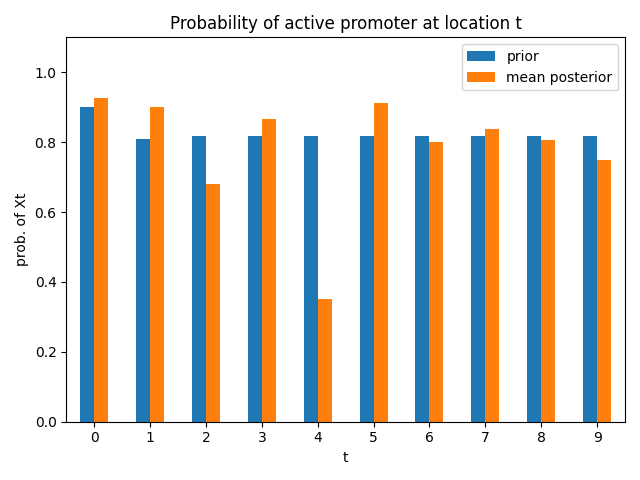
\includegraphics[width=0.4\textwidth]{../plots/q1_prior_vs_mean_posterior.png}
        \caption{Prior distributions $p(X_t = 1)$ versus the mean marginal posteriors $\mu_t = \frac{1}{N} \sum_{i=1}^{N} p(X_t = 1 | o_{1:T}[i])$ for each $t$.}
    \end{figure}

    
    The plot shows the prior distributions $p(X_t = 1)$ (blue bars) versus the mean marginal posteriors $\mu_t$ 
    (orange bars) for each time step $t$. The differences between the prior and the mean marginal posteriors suggest
     that the observations have a significant impact on the estimated probabilities of active promoters. 
     Specifically, the mean marginal posteriors differ from the prior distributions due to the evidence provided 
     by the observations. This indicates that the dataset likely contains informative observations that influence the 
     posterior estimates. \\
     The deviations from the prior suggest that the distribution from which the observations were sampled has regions with
      varying levels of promoter activity, as captured by the posterior probabilities.
    

    \item \tblu{We want to use the marginal posteriors $p(X_t | o_{1:T}[i])$ to assign each location $t$ its status and predict areas of active promoter:
    \[
    \hat{X}_t[i] = \arg\max_x p(X_t = x | o_{1:T}[i])
    \]
    Implement a \texttt{naive\_predict\_by\_posterior} method in the HMM class.}

    Implemented the \texttt{naive\_predict\_by\_posterior} method in the HMM class.
    

    \item \tblu{Prediction:
    We use this method to predict hidden sequences for the given observations. We compare them to the ground-truth sequences from \texttt{hidden\_data.csv}.
     What is the accuracy of these predictions (use the same definition as Project 1)? What is the difference compared to the prediction we used in Project 1?
      Is the rule in Eq.4 a good prediction rule?}

    \textbf{Results:}
    \begin{itemize}
        \item Exact Posterior Prediction Accuracy: 0.900
        \item Naive Prediction Accuracy: 0.895
    \end{itemize}
    
    \textbf{Analysis:}
    \begin{itemize}
        \item The exact posterior method is slightly more accurate than the naive method.
        \item The exact method uses the forward-backward algorithm, considering the entire observation sequence, 
            while the naive method likely uses a simpler, less contextual approach.
        \item This accuracy difference shows the exact posterior is better at capturing dependencies in the data.
        \item Eq. 4's rule is a good prediction method, leveraging the full observation sequence for more informed predictions.
    \end{itemize}

\end{enumerate}

\subsection*{2. Sampling-based inference}


\begin{enumerate}
    \item \tblu{Gibbs sampling: In this algorithm, we’ll start with a starting point $X_{1:T}$ sampled from the prior $p(X_{1:T})$, 
    and sample $M$ sequences of hidden states sequentially:
    \[
    X_t^{(m)} \sim p(X_t | X_{-t}^{(m-1)}, o_{1:T}[i]), \quad t = 1, \ldots, T
    \]
    We then use the samples to estimate the posterior $p(X_t = x | o_{1:T}[i])$ for each $t$.}
    
    \begin{enumerate}
        \item \tblu{For observations $o_{1:T}[i]$, at iteration $m$, we want to use the samples from the previous iteration 
        $\{X_t^{(m-1)}\}_{t=1}^{T}$ to sample $X_t^{(m)}$ from the distribution $p(X_t | X_{-t}^{(m-1)}, o_{1:T}[i])$. 
        How can we sample from this distribution using the CPDs of the network?} \\

        In a Hidden Markov Model (HMM), the Markov blanket of a hidden state $X_t$ includes its immediate neighbors and the observation at time $t$. Specifically, the Markov blanket of $X_t$ consists of $X_{t-1}$, $O_t$, and $X_{t+1}$ (if they exist). This is because in an HMM, $X_t$ is conditionally independent of all other variables given these three variables. 

        Given this, we can write the conditional distribution for sampling $X_t$ as follows:

        \begin{align*}
            &P(X_t = k \mid X_{-t}^{(m-1)}, O_{1:T}[i]) \\
            &= P(X_t = k \mid X_{t-1}^{(m-1)}, O_t[i], X_{t+1}^{(m-1)}) \\
            &= \frac{P_\phi(X_t = k, X_{t-1}^{(m-1)}, O_t[i], X_{t+1}^{(m-1)})}{\sum_{x_t \in \text{Val}(X_t)} P_\phi(X_t = x_t, X_{t-1}^{(m-1)}, O_t[i], X_{t+1}^{(m-1)})} \\
            &= \frac{P_\phi(X_{t-1}^{(m-1)}) \cdot P(X_t = k \mid X_{t-1}^{(m-1)}) \cdot P(O_t[i] \mid X_t = k) \cdot P(X_{t+1}^{(m-1)} \mid X_t = k)}{\sum_{x_t \in \text{Val}(X_t)} P_\phi(X_{t-1}^{(m-1)}) \cdot P(X_t = x_t \mid X_{t-1}^{(m-1)}) \cdot P(O_t[i] \mid X_t = x_t) \cdot P(X_{t+1}^{(m-1)} \mid X_t = x_t)} \\
            &= \frac{P(X_t = k \mid X_{t-1}^{(m-1)}) \cdot P(O_t[i] \mid X_t = k) \cdot P(X_{t+1}^{(m-1)} \mid X_t = k)}{\sum_{x_t \in \text{Val}(X_t)} P(X_t = x_t \mid X_{t-1}^{(m-1)}) \cdot P(O_t[i] \mid X_t = x_t) \cdot P(X_{t+1}^{(m-1)} \mid X_t = x_t)}
        \end{align*}

        
        \item \tblu{Given $M$ samples $\{X_t^{(m)}\}_{m=1}^{M}$ from the process described above, 
        how can we calculate the posterior $p(X_t = x | o_{1:T}[i])$, while discarding the first $M_{\text{start}}$ samples to allow for a “burn-in” period?}

        To calculate the posterior $p(X_t = x | o_{1:T}[i])$ for each $t$, we can use the samples $\{X_t^{(m)}\}_{m=M_{\text{start}}}^{M}$
        obtained from the Gibbs sampling process. 
        We can estimate the posterior by counting the number of times $X_t = x$ occurs in the samples and normalizing by the total number of samples. 
        The posterior can be calculated as follows:

        \[
        p(X_t = x | o_{1:T}[i]) = \frac{1}{M - M_{\text{start}}} \sum_{m=M_{\text{start}}}^{M} \mathbb{I}(X_t^{(m)} = x)
        \]

        where $\mathbb{I}(\cdot)$ is the indicator function that returns 1 if the condition is true and 0 otherwise.
        
        \item \tblu{Implement a method \texttt{gibbs\_sampling\_posterior} in the HMM class to calculate the posterior 
        $p(X_t = x | o_{1:T}[i])$ for each $t$ with $M - M_{\text{start}}$ samples.}
        

        Implemented the \texttt{gibbs\_sampling\_posterior} method in the HMM class.


        \item \tblu{We run the Gibbs algorithm with $M \in [10, 50, 70, 100, 200, 300, 500]$ samples to calculate the marginal 
        posteriors of each observation in the dataset. We run the algorithm 5 times for each value of $M$. 
        We plot the posterior of $X_5$ for the first 10 observations $p(X_5 | o_{1:T}[1 : 10])$ versus $M$ with confidence 
        intervals ($\mu \pm \sigma$), and add to the plot the exact posterior calculated using DP.
        Does the Gibbs estimation converge? Does it converge to the correct posterior? Explain your results. 
        What can you say about the convergence of this algorithm?}

        \begin{figure}[H]
            \centering
            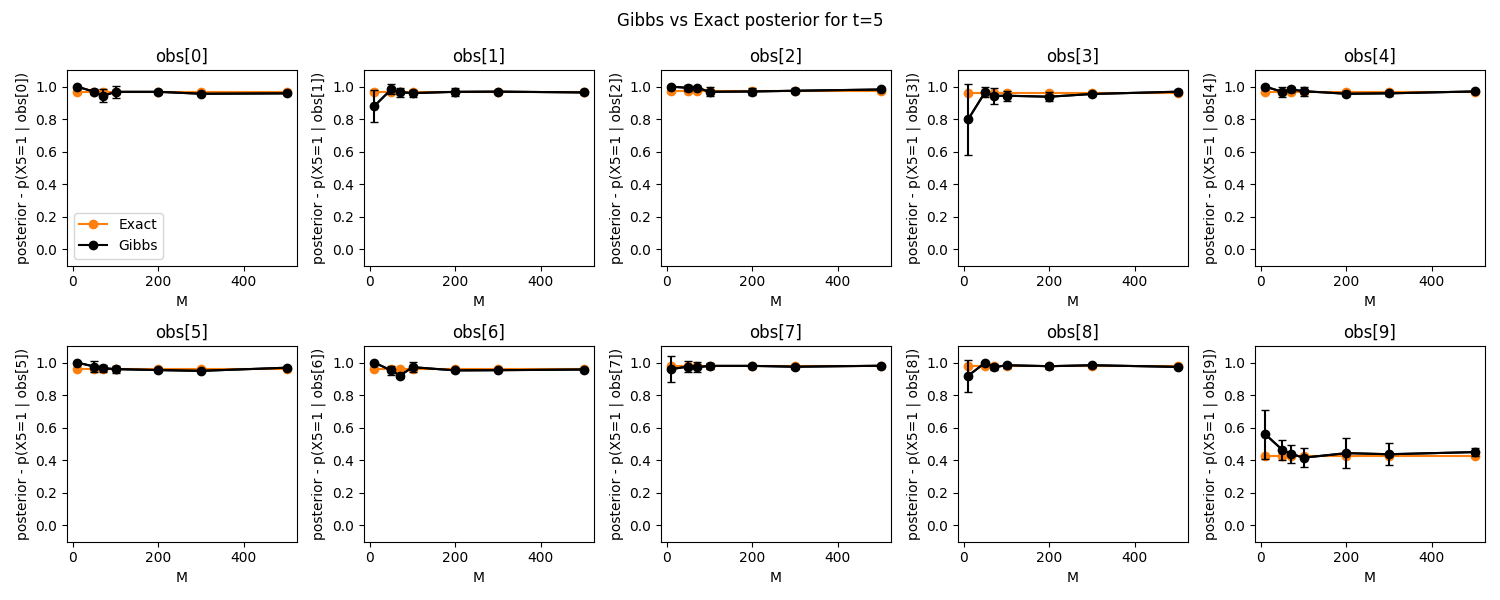
\includegraphics[width=0.9\textwidth]{../plots/Gibbs_est_vs_exact_posterior.png}
            \caption{Posterior of $X_5$ for the first 10 observations $p(X_5 | o_{1:T}[1 : 10])$ versus $M$ with confidence intervals ($\mu \pm \sigma$).}
        \end{figure}

        The plot shows the comparison between the Gibbs sampling estimation and the exact posterior calculated 
        using dynamic programming (DP) for $X_5$ across the first 10 observations. 

        \textbf{Analysis:}
        \begin{itemize}
            \item \textbf{Convergence:} The Gibbs estimation converges fairly fast as $M$ increases. Even with a relatively small number of samples (e.g., $M = 50$), the estimates are quite stable and close to the exact posterior.
            \item \textbf{Correctness:} The Gibbs estimates converge to values close to the exact posterior calculated using DP, indicating that the Gibbs sampling method is correctly estimating the posterior distributions.
            \item \textbf{Results:} The convergence of the Gibbs sampling algorithm demonstrates its effectiveness in approximating the true posterior distribution, especially with a higher number of samples $M$. The confidence intervals also decrease with increasing $M$, showing more precise estimates.
            \item \textbf{Implications:} The fast convergence of the Gibbs sampling method makes it a practical and efficient approach for posterior estimation in HMMs, providing reliable results with relatively few samples.
        \end{itemize}
        
    \end{enumerate}
    
    \item \tblu{We use the estimated posteriors of each algorithm and the \texttt{naive\_predict\_by\_posterior} method to assign 
    each location its status (same as for the exact posterior). We plot the accuracy of the algorithms as a function of $M$, 
    and plot on the same graph the accuracy of the exact posterior (as a constant function of $M$). What is the trend?}


    \begin{figure}[H]
        \centering
        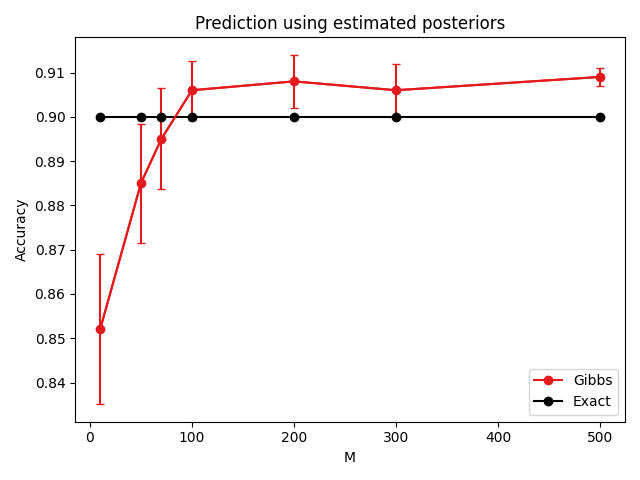
\includegraphics[width=0.6\textwidth]{../plots/est_vs_exact_accuracy.png}
        \caption{Accuracy of the algorithms as a function of $M$, with the accuracy of the exact posterior as a constant function of $M$.}
    \end{figure}

    The plot shows the accuracy of the Gibbs sampling algorithm compared to the exact posterior as a function of the number of samples $M$.

    \textbf{Analysis:}
    \begin{itemize}
        \item \textbf{Trend:} The accuracy of the Gibbs sampling algorithm increases rapidly with the number of samples $M$ and stabilizes around $M = 100$. The exact posterior accuracy remains constant.
        \item \textbf{Comparison:} The Gibbs sampling method eventually reaches and slightly surpasses the accuracy of the exact posterior, indicating that it is an effective method for estimating the posterior, especially with a larger number of samples.
        \item \textbf{Implications:} The Gibbs sampling method can achieve high accuracy with sufficient samples, making it a reliable alternative to exact inference methods. The slight fluctuation in accuracy with smaller $M$ values suggests that more samples are needed for stabilization.
    \end{itemize}

\end{enumerate}

\end{document}




